\documentclass{article}
\usepackage[utf8]{inputenc}
\usepackage{tikz}
\usetikzlibrary {positioning}
\usetikzlibrary {arrows.meta,automata,positioning,shadows}




\title{Assignment 10}
\author{Perisetti Sai Ram Mohan Rao}
\begin{document}


\maketitle

\section{Question 1}
The state diagram of Finite State Machine (FSM) desgined to detect an overlapping sequence of three bits as shown in figure. The FSM has an input 'In' and an output 'Out'.The intial state of FSM is $S_0$ .

\begin{figure}[h]
\centering
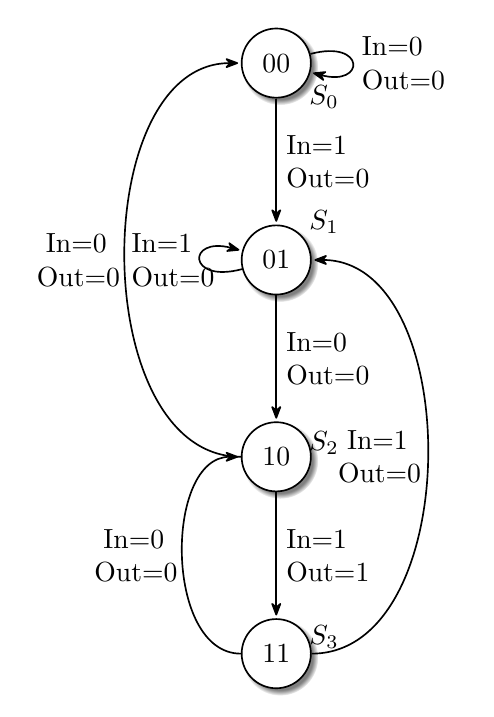
\begin{tikzpicture}[->,>={Stealth[round]},shorten >=1pt,auto,node distance=2.5cm,on grid,semithick,
every state/.style={fill=white,draw=black,circular drop shadow,text=}]
\node[state] (A)               {00};
\node[state] (B) [below =of A] {01};
\node[state] (C) [below =of B] {10};
\node[state] (D) [below =of C] {11};
\put (12,-15) {$S_0$};
\put (12,-60) {$S_1$};
\put (12,-140) {$S_2$};
\put (12,-210) {$S_3$};




\path (A) edge [loop right]   node[text width=0.75cm,align=center]{In=0\\Out=0}(A)
      (A) edge                node[text width=0.75cm,align=center]{In=1\\Out=0} (B)
      (B) edge [loop left]   node[text width=0.75cm,align=center]{In=1\\Out=0} (B)
      (B) edge                node[text width=0.75cm,align=center]{In=0\\Out=0} (C)
      (C) edge                node[text width=0.75cm,align=center]{In=1\\Out=1} (D)
      (D) edge [bend left=90]    node[text width=1.00cm,align=center]{In=0\\Out=0} (C)
      (C) edge [bend left=90] node[text width=1.0cm,align=center]{In=0\\Out=0} (A)
      (D) edge [bend right=90] node[text width=1.0cm,align=center]{In=1\\Out=0} (B);


\end{tikzpicture}


\caption{}
\label{figure}
\end{figure}

If the input sequence is 10101101001101, starting with leftmost bit,then how many number of times 'Out' will be 1 is \rule{2cm}{0.10mm}

\maketitle 

\section{Solution}
We are requried to find output sequence of Finite State Machine(FSM) and number 1's in output sequence.

\begin{figure}[h]
\centering
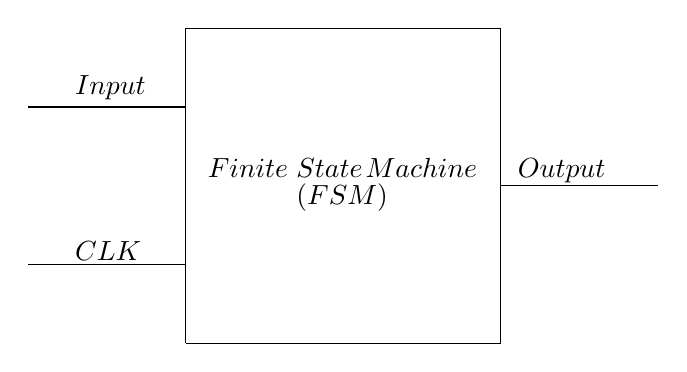
\begin{tikzpicture}

\draw (0,1)--(-2,1);
\draw (0,3)--(-2,3);
\draw (0,0) -- (4,0) -- (4,4) -- (0,4) -- (0,0);
\draw (4,2)--(6,2);
\put  (-40,90) {$Input$}
\put  (-40,30) {$CLK$}
\put  (8,60) {$Finite$}
\put  (40,60) {$State$}
\put  (65,60) {$Machine$}
\put  (40,50) {$(FSM)$}
\put  (120,60) {$Output$}

\end{tikzpicture}


\caption{}
\label{figure}
\end{figure}

If the CLK is not applied,there will be no differnce between input sequence and the output sequence.

The mechanism that should take place in Finite state machine is mentioned in Figure 1.We will take few parts of figure in question.

\begin{figure}[h]
\centering
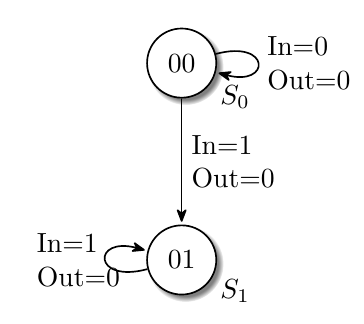
\begin{tikzpicture}[->,>={Stealth[round]},shorten >=1pt,auto,node distance=2.5cm,on grid,semithick,
every state/.style={fill=white,draw=black,circular drop shadow,text=}]
\node[state] (A)               {00};
\node[state] (B) [below =of A] {01};

\put (14,-15) {$S_0$};
\put (14,-85) {$S_1$};





\path (A) edge [loop right]   node[text width=0.75cm,align=center]{In=0\\Out=0}(A)
      (A) edge                node[text width=0.75cm,align=center]{In=1\\Out=0} (B)
      (B) edge [loop left]   node[text width=0.75cm,align=center]{In=1\\Out=0} (B);


\end{tikzpicture}
\caption{}
\label{figure}
\end{figure}


\begin{figure}[h]
\centering
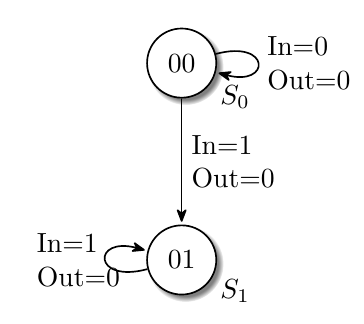
\begin{tikzpicture}[->,>={Stealth[round]},shorten >=1pt,auto,node distance=2.5cm,on grid,semithick,
every state/.style={fill=white,draw=black,circular drop shadow,text=}]
\node[state] (A)               {00};
\node[state] (B) [below =of A] {01};

\put (14,-15) {$S_0$};
\put (14,-85) {$S_1$};





\path (A) edge [loop right]   node[text width=0.75cm,align=center]{In=0\\Out=0}(A)
      (A) edge                node[text width=0.75cm,align=center]{In=1\\Out=0} (B)
      (B) edge [loop left]   node[text width=0.75cm,align=center]{In=1\\Out=0} (B);


\end{tikzpicture}
\caption{}
\label{figure}
\end{figure}


In the finite machine we are requried to find the output in current state for corresponding input .We have to see Input value at current state to get the Output.For example if we are at current state $S_0$ with input=1 then Output =0 and state changes to $S_1$.



We are now looking at another example.If the current state of FSM is $S_2$ with input=0
then it gives output=0 and state changes to $S_0$.


Output sequence of corresponding current state of given input sequence is 00101001000001
that is repesented in Table 1 Current state,Input and output.


\begin{table}[h]
\centering
\begin{tabular}{|c|c|c|c|c|c|c|c|c|c|c|c|c|c|c|c|}
\hline
\textit{\textbf{Current State}} &\textit{\textbf{$S_0$}}  & \textit{\textbf{$S_1$}} & \textit{\textbf{$S_2$}} & \textit{\textbf{$S_3$}}&\textit{\textbf{$S_2$}} &\textit{\textbf{$S_3$}} &\textit{$S_1$} &\textit{$S_2$} &\textit{$S_3$} &\textit{$S_2$} &\textit{$S_0$} &\textit{$S_1$} &\textit{$S_1$}&\textit{$S_2$}  \\\hline
\textit{\textbf{Input}}         &    1                   &    0                    &   1                     &   0                    &   1                    &   1                    &   0            &   1           &   0           &   0           &   1           &   1           &   0          &    1            \\\hline
\textit{\textbf{Output}}        &    0                   &    0                    &   1                     &   0                    &   1                    &   0                    &   0            &   1           &   0           &   0           &   0           &   0           &   0          &    1           \\\hline
\end{tabular}
\caption{Table for States,Input and Output of finite state machine}
\label{table}
\end{table}

The Output sequence of FSM is 00101001000001 from Table 1. \\
Then number of times 'Out' will be 1 is 4

\centering 
Answer = 4

\end{document}
